

Os usuários finais do sistema EnTurma possuem como maior necessidade a de visualizar o desempenho de uma determinada turma do sistema educacional brasileiro. A tabela \ref{tab:recursos} apresenta todos os recursos do sistema e suas características.

\begin{table}[H]
	\centering
	\begin{tabular}{|l|l|}
		\hline
		\textbf{Necessidade}      & \textbf{Características}                                                                                                                                                                                                                                                                                                   \\ \hline
		Gerar relatório da turma  & \begin{tabular}[c]{@{}l@{}}Os gráficos podem ser gerados a partir dos indicadores \\ e período escolhidos. Os indicadores podem ser: média\\  dos alunos, média de horas/aula, taxa de rendimento, \\ e outros. O período escolhido pode variar entre 2006 a \\ 2014 dependendo da disponibilidade dos dados.\end{tabular} \\ \hline
		Comparar turmas           & \begin{tabular}[c]{@{}l@{}}Comparação de duas turmas em um mesmo indicador. \\ Exemplo: comparar a turma da primeira série do ano \\ de 2007 com a de 2008 em relação à média escolar.\end{tabular}                                                                                                                        \\ \hline
		Gerar ranking             & \begin{tabular}[c]{@{}l@{}}O sistema deve gerar ranking dos melhores estados em \\ um determinado indicador.\end{tabular}                                                                                                                                                                                                  \\ \hline
		Contactar desenvolvedores & \begin{tabular}[c]{@{}l@{}}O sistema disponibiliza uma seção que permite que o \\ usuário entre em contato com os desenvolvedores a fim \\ de sanar dúvidas, fazer críticas ou sugestões sobre o sistema.\end{tabular}                                                                                                     \\ \hline
	\end{tabular}
	\caption{Recursos do Sistema}
	\label{tab:recursos}
\end{table}

	O relacionamento destes recursos com os Atores do sistema pode ser observado na Modelagem de Casos de Uso do Sistema Enturma, que está disposta na figura \ref{img:modelagem}.

	\begin{figure}[H]
		\centering
		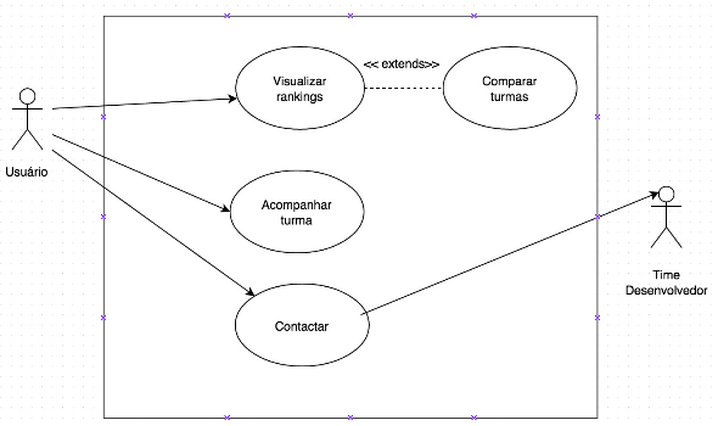
\includegraphics[width=0.7\textwidth]{imagens/modelagem}
		\caption{Modelagem de Casos de Uso}
		\label{img:modelagem}
	\end{figure}

